\newcommand{\brainageplot}[1]{
    \begin{tikzpicture}
        \begin{axis}[
            height=5cm,
            width=5cm,
            xlabel=\small{Chronological age},
            ylabel=\small{Apparent brain age},
            xmin=0,
            xmax=100,
            ymin=0,
            ymax=100,
            ticklabel style={font=\small},
            ylabel style={yshift=-0.2cm},
            xlabel style={yshift=0.05cm},
            ytick pos=left,
            xtick pos=bottom
        ]
            \addplot[dashed] coordinates {(0, 0) (100, 100)};

            \ifnum#1=0
                \node[rotate=45, anchor=north, inner sep=1pt] at (axis cs: 48, 48) {
                    \tiny{Normative aging trajectory}
                };
            \fi

            \ifnum#1=1
                \draw[-stealth,densely dotted] (axis cs: 30, 30) -- (axis cs: 30, 48);
                \draw[-stealth,densely dotted] (axis cs: 70, 70) -- (axis cs: 70, 57);
                \addplot[
                    only marks,
                    mark=*,
                    draw=blue,
                    fill=blue!50
                ] coordinates {
                    (30, 50)
                    (70, 55)
                };
                \node[
                    font=\scriptsize\linespread{0.8}\selectfont,
                    anchor=south,
                    align=center
                ] at (axis cs: 30, 50) {
                    Older\\looking\\brain
                };
                \node[
                    font=\scriptsize\linespread{0.8}\selectfont,
                    anchor=north,
                    align=center
                ] at (axis cs: 70, 55) {
                    Younger\\looking\\brain
                };

            \fi
        \end{axis}
    \end{tikzpicture}
}

\newsavebox{\brainage}
\sbox{\brainage}{
    \brainageplot{0}
}

\newsavebox{\brainagepredictions}
\sbox{\brainagepredictions}{
    \brainageplot{1}
}

\newcommand{\brainagedataset}{
    \definecolor{hbn-clr}{RGB}{255, 0, 40}
    \definecolor{adhd200-clr}{RGB}{255, 27, 0}
    \definecolor{ping-clr}{RGB}{255, 96, 0}
    \definecolor{ds000119-clr}{RGB}{255, 165, 0}
    \definecolor{abide-clr}{RGB}{255, 234, 0}
    \definecolor{slim-clr}{RGB}{206, 255, 0}
    \definecolor{abide2-clr}{RGB}{137, 255, 0}
    \definecolor{beijing-clr}{RGB}{68, 255, 0}
    \definecolor{aomic-clr}{RGB}{0, 255, 0}
    \definecolor{corr-clr}{RGB}{0, 255, 68}
    \definecolor{mpi-clr}{RGB}{0, 255, 137}
    \definecolor{hcp-clr}{RGB}{0, 255, 205}
    \definecolor{fcon-clr}{RGB}{0, 235, 255}
    \definecolor{nki-clr}{RGB}{0, 166, 255}
    \definecolor{sald-clr}{RGB}{0, 97, 255}
    \definecolor{ds000222-clr}{RGB}{0, 27, 255}
    \definecolor{dlbs-clr}{RGB}{41, 0, 255}
    \definecolor{camcan-clr}{RGB}{110, 0, 255}
    \definecolor{ukb-clr}{RGB}{180, 0, 255}
    \definecolor{oasis-clr}{RGB}{249, 0, 255}
    \definecolor{ds000202-clr}{RGB}{255, 0, 191}

    \begin{tikzpicture}
        \begin{axis}[
            width=0.9\textwidth,
            height=0.65\textwidth,
            xmin=0,
            xmax=100,
            ymin=-1200,
            ymax=1200,
            yticklabels={,,},
            ytick=\empty,
            xtick pos=bottom,
            y dir=reverse,
            axis x line=middle,
            axis y line=none,
            xtick={0,10,20,30,40,50,60,70,80}
        ]
            \addplot [draw=none, name path=zero] coordinates {
                (0, 0)
                (100, 0)
            };

            \addplot [draw=none, name path=hbn] table [col sep=comma, x=age,y=hbn] {data/brain_age/dataset/M.csv};
            \addplot [hbn-clr] fill between [of=zero and hbn];
            \addplot [draw=none, name path=adhd200] table [col sep=comma, x=age,y=adhd200-hc] {data/brain_age/dataset/M.csv};
            \addplot [adhd200-clr] fill between [of=hbn and adhd200];\label{trace:adhd200}
            \addplot [draw=none, name path=ping] table [col sep=comma, x=age,y=ping] {data/brain_age/dataset/M.csv};
            \addplot [ping-clr] fill between [of=adhd200 and ping];\label{trace:ping}

            \addplot [draw=none, name path=ds000119] table [col sep=comma, x=age,y=ds000119] {data/brain_age/dataset/M.csv};
            \addplot [ds000119-clr] fill between [of=ping and ds000119];\label{trace:ds000119}
            \addplot [draw=none, name path=abide] table [col sep=comma, x=age,y=abide-hc] {data/brain_age/dataset/M.csv};
            \addplot [abide-clr] fill between [of=ds000119 and abide];\label{trace:abide}
            \addplot [draw=none, name path=slim] table [col sep=comma, x=age,y=slim] {data/brain_age/dataset/M.csv};
            \addplot [slim-clr] fill between [of=abide and slim];\label{trace:slim}
            \addplot [draw=none, name path=abide2] table [col sep=comma, x=age,y=abide2-hc] {data/brain_age/dataset/M.csv};
            \addplot [abide2-clr] fill between [of=slim and abide2];\label{trace:abide2}
            \addplot [draw=none, name path=beijing] table [col sep=comma, x=age,y=beijing-enhanced] {data/brain_age/dataset/M.csv};
            \addplot [beijing-clr] fill between [of=slim and beijing];\label{trace:beijing}
            \addplot [draw=none, name path=aomic] table [col sep=comma, x=age,y=aomic-id1000] {data/brain_age/dataset/M.csv};
            \addplot [aomic-clr] fill between [of=beijing and aomic];\label{trace:aomic}
            \addplot [draw=none, name path=corr] table [col sep=comma, x=age,y=corr] {data/brain_age/dataset/M.csv};
            \addplot [corr-clr] fill between [of=aomic and corr];\label{trace:corr}
            \addplot [draw=none, name path=mpi] table [col sep=comma, x=age,y=mpi-lemon] {data/brain_age/dataset/M.csv};
            \addplot [mpi-clr] fill between [of=corr and mpi];\label{trace:mpi}
            \addplot [draw=none, name path=hcp] table [col sep=comma, x=age,y=hcp] {data/brain_age/dataset/M.csv};
            \addplot [hcp-clr] fill between [of=mpi and hcp];\label{trace:hcp}
            \addplot [draw=none, name path=fcon] table [col sep=comma, x=age,y=fcon1000] {data/brain_age/dataset/M.csv};
            \addplot [fcon-clr] fill between [of=hcp and fcon];\label{trace:fcon}
            \addplot [draw=none, name path=nki] table [col sep=comma, x=age,y=nki-rockland] {data/brain_age/dataset/M.csv};
            \addplot [nki-clr] fill between [of=fcon and nki];\label{trace:nki}
            \addplot [draw=none, name path=sald] table [col sep=comma, x=age,y=sald] {data/brain_age/dataset/M.csv};
            \addplot [sald-clr] fill between [of=nki and sald];\label{trace:sald}
            \addplot [draw=none, name path=ds000222] table [col sep=comma, x=age,y=ds000222] {data/brain_age/dataset/M.csv};
            \addplot [ds000222-clr] fill between [of=sald and ds000222];\label{trace:ds000222}
            \addplot [draw=none, name path=dlbs] table [col sep=comma, x=age,y=dlbs] {data/brain_age/dataset/M.csv};
            \addplot [dlbs-clr] fill between [of=ds000222 and dlbs];\label{trace:dlbs}
            \addplot [draw=none, name path=camcan] table [col sep=comma, x=age,y=camcan] {data/brain_age/dataset/M.csv};
            \addplot [camcan-clr] fill between [of=dlbs and camcan];\label{trace:camcan}
            \addplot [draw=none, name path=ukb] table [col sep=comma, x=age,y=ukb] {data/brain_age/dataset/M.csv};
            \addplot [ukb-clr] fill between [of=camcan and ukb];\label{trace:ukb}
            \addplot [draw=black, name path=oasis] table [col sep=comma, x=age,y=oasis3-hc] {data/brain_age/dataset/M.csv};
            \addplot [oasis-clr] fill between [of=ukb and oasis];\label{trace:oasis}

            \addplot [draw=none, name path=hbn] table [col sep=comma, x=age,y expr=\thisrow{hbn}*-1] {data/brain_age/dataset/F.csv};
            \addplot [hbn-clr] fill between [of=zero and hbn];\label{trace:hbn}
            \addplot [draw=none, name path=adhd200] table [col sep=comma, x=age,y=,y expr=\thisrow{adhd200-hc}*-1] {data/brain_age/dataset/F.csv};
            \addplot [adhd200-clr] fill between [of=hbn and adhd200];
            \addplot [draw=none, name path=ping] table [col sep=comma, x=age,y expr=\thisrow{ping}*-1] {data/brain_age/dataset/F.csv};
            \addplot [ping-clr] fill between [of=adhd200 and ping];
            \addplot [draw=none, name path=abide] table [col sep=comma, x=age,y expr=\thisrow{abide-hc}*-1] {data/brain_age/dataset/F.csv};
            \addplot [abide-clr] fill between [of=ping and abide];
            \addplot [draw=none, name path=abide2] table [col sep=comma, x=age,y expr=\thisrow{abide2-hc}*-1] {data/brain_age/dataset/F.csv};
            \addplot [abide2-clr] fill between [of=abide and abide2];
            \addplot [draw=none, name path=ds000119] table [col sep=comma, x=age,y=,y expr=\thisrow{ds000119}*-1] {data/brain_age/dataset/F.csv};
            \addplot [ds000119-clr] fill between [of=abide2 and ds000119];
            \addplot [draw=none, name path=slim] table [col sep=comma, x=age,y expr=\thisrow{slim}*-1] {data/brain_age/dataset/F.csv};
            \addplot [slim-clr] fill between [of=ds000119 and slim];
            \addplot [draw=none, name path=beijing] table [col sep=comma, x=age,y expr=\thisrow{beijing-enhanced}*-1] {data/brain_age/dataset/F.csv};
            \addplot [beijing-clr] fill between [of=slim and beijing];
            \addplot [draw=none, name path=ds000202] table [col sep=comma, x=age,y expr=\thisrow{ds000202}*-1] {data/brain_age/dataset/F.csv};
            \addplot [ds000202-clr] fill between [of=beijing and ds000202];\label{trace:ds000202}
            \addplot [draw=none, name path=aomic] table [col sep=comma, x=age,y expr=\thisrow{aomic-id1000}*-1] {data/brain_age/dataset/F.csv};
            \addplot [aomic-clr] fill between [of=beijing and aomic];
            \addplot [draw=none, name path=mpi] table [col sep=comma, x=age,y expr=\thisrow{mpi-lemon}*-1] {data/brain_age/dataset/F.csv};
            \addplot [mpi-clr] fill between [of=aomic and mpi];
            \addplot [draw=none, name path=corr] table [col sep=comma, x=age,y expr=\thisrow{corr}*-1] {data/brain_age/dataset/F.csv};
            \addplot [corr-clr] fill between [of=mpi and corr];
            \addplot [draw=none, name path=fcon] table [col sep=comma, x=age,y expr=\thisrow{fcon1000}*-1] {data/brain_age/dataset/F.csv};
            \addplot [fcon-clr] fill between [of=corr and fcon];
            \addplot [draw=none, name path=hcp] table [col sep=comma, x=age, y expr=\thisrow{hcp}*-1] {data/brain_age/dataset/F.csv};
            \addplot [hcp-clr] fill between [of=fcon and hcp];
            \addplot [draw=none, name path=nki] table [col sep=comma, x=age,y expr=\thisrow{nki-rockland}*-1] {data/brain_age/dataset/F.csv};
            \addplot [nki-clr] fill between [of=hcp and nki];
            \addplot [draw=none, name path=ds000222] table [col sep=comma, x=age,y expr=\thisrow{ds000222}*-1] {data/brain_age/dataset/F.csv};
            \addplot [ds000222-clr] fill between [of=nki and ds000222];
            \addplot [draw=none, name path=sald] table [col sep=comma, x=age,y expr=\thisrow{sald}*-1] {data/brain_age/dataset/F.csv};
            \addplot [sald-clr] fill between [of=ds000222 and sald];
            \addplot [draw=none, name path=camcan] table [col sep=comma, x=age,y expr=\thisrow{camcan}*-1] {data/brain_age/dataset/F.csv};
            \addplot [camcan-clr] fill between [of=sald and camcan];
            \addplot [draw=none, name path=dlbs] table [col sep=comma, x=age,y expr=\thisrow{dlbs}*-1] {data/brain_age/dataset/F.csv};
            \addplot [dlbs-clr] fill between [of=camcan and dlbs];

            \addplot [draw=none, name path=ukb] table [col sep=comma, x=age,y expr=\thisrow{ukb}*-1] {data/brain_age/dataset/F.csv};
            \addplot [ukb-clr] fill between [of=dlbs and ukb];
            \addplot [draw=black, name path=oasis] table [col sep=comma, x=age,y expr=\thisrow{oasis3-hc}*-1] {data/brain_age/dataset/F.csv};
            \addplot [oasis-clr] fill between [of=ukb and oasis];

            \addplot [] coordinates {
                (0, 0)
                (100, 0)
            };
            \coordinate (male) at (axis cs:100,35) {};
            \coordinate (female) at (axis cs:100,-35) {};

            \node[] at (50,1056) {\textbf{\footnotesize{n=53542}}};
        \end{axis}
        \matrix [
            draw=none,
            matrix of nodes,
            anchor=north west,
            row sep=-0.2cm,
            font=\scriptsize,
            column 1/.style={anchor=base west}
        ] at (8.2, 6.31) {
            \ref{trace:hbn} HBN \\
            \ref{trace:adhd200} ADHD200 \\
            \ref{trace:ping} PING \\
            \ref{trace:ds000119} ds000119 \\
            \ref{trace:abide} ABIDE \\
            \ref{trace:slim} SLIM \\
            \ref{trace:abide2} ABIDE2 \\
            \ref{trace:beijing} Beijing \\
            \ref{trace:aomic} AOMIC \\
            \ref{trace:corr} CoRR \\
            \ref{trace:mpi} MPI-Lemon \\
            \ref{trace:hcp} HCP \\
            \ref{trace:fcon} FCON1000 \\
            \ref{trace:nki} NKI Rockland \\
            \ref{trace:sald} SALD \\
            \ref{trace:ds000222} ds000222 \\
            \ref{trace:dlbs} DLBS \\
            \ref{trace:camcan} CamCAN \\
            \ref{trace:ukb} UKB \\
            \ref{trace:oasis} OASIS3 \\
            \ref{trace:ds000202} ds000202 \\
        };
        \node [anchor=north east] at (male) {\footnotesize{MALE}};
        \node [anchor=south east] at (female) {\footnotesize{FEMALE}};
    \end{tikzpicture}
}

\newcommand{\brainageresults}{
    \begin{tikzpicture}
        \begin{groupplot}[
            group style={
                group size=2 by 1,
                horizontal sep=1.2cm,
                vertical sep=0.8cm
            },
            width=0.5\linewidth,
            height=0.5\linewidth
        ]

            \nextgroupplot[
                xmin=0,
                xmax=100,
                ymin=0,
                ymax=100,
                xtick pos=bottom,
                ytick pos=left,
                ticklabel style = {font=\footnotesize},
                xlabel=\footnotesize{Chronological age},
                ylabel=\footnotesize{Predicted brain age},
                title={Test set}
            ]
                \addplot [red] coordinates {(0,0) (100,100)};
                \addplot [
                    only marks,
                    mark size=1.5pt,
                    color=black,
                    opacity=0.35
                ] table [
                    x=regression,
                    y=age,
                    each nth point={10},
                    col sep=comma
                ] {data/brain_age/prediction/test_predictions.csv};
                \node [anchor=south east,inner sep=0pt,outer sep=0pt] (outofsample) at (rel axis cs:0.92,0.08) {\footnotesize{\textcolor{red}{MAE=2.47}}};

        %     \nextgroupplot[
        %         xmin=0,
        %         xmax=100,
        %         ymin=0,
        %         ymax=100,
        %         xtick pos=bottom,
        %         ytick pos=left,
        %         ticklabel style = {font=\footnotesize},
        %         title={External test set}
        %     ]
        %         \addplot [red] coordinates {(0,0) (100,100)};
        %         \addplot [
        %             only marks,
        %             mark size=1.5pt,
        %             color=black,
        %             opacity=0.35
        %         ] table [
        %             x=regression,
        %             y=age,
        %             each nth point={\N},
        %             col sep=comma
        %         ] {data/brain_age/prediction/external_predictions.csv};
        %         \node [anchor=south east,inner sep=0pt,outer sep=0pt] (outofsample) at (rel axis cs:0.92,0.08) {\footnotesize{\textcolor{red}{MAE=3.90}}};
        \end{groupplot}
    \end{tikzpicture}
}

\begin{frame}{Brain age predictions using deep learning}
    \begin{tikzpicture}
        \node[] at (-5.25, 3.5) {};
        \node[] at (5.25, -3.5) {};

        \visible<1-3>{
            \node[anchor=west, label={[label distance=-0.15cm, anchor=north]below:\scriptsize{Generated by Dall-E 3}}] at (-5.1, 0) {
                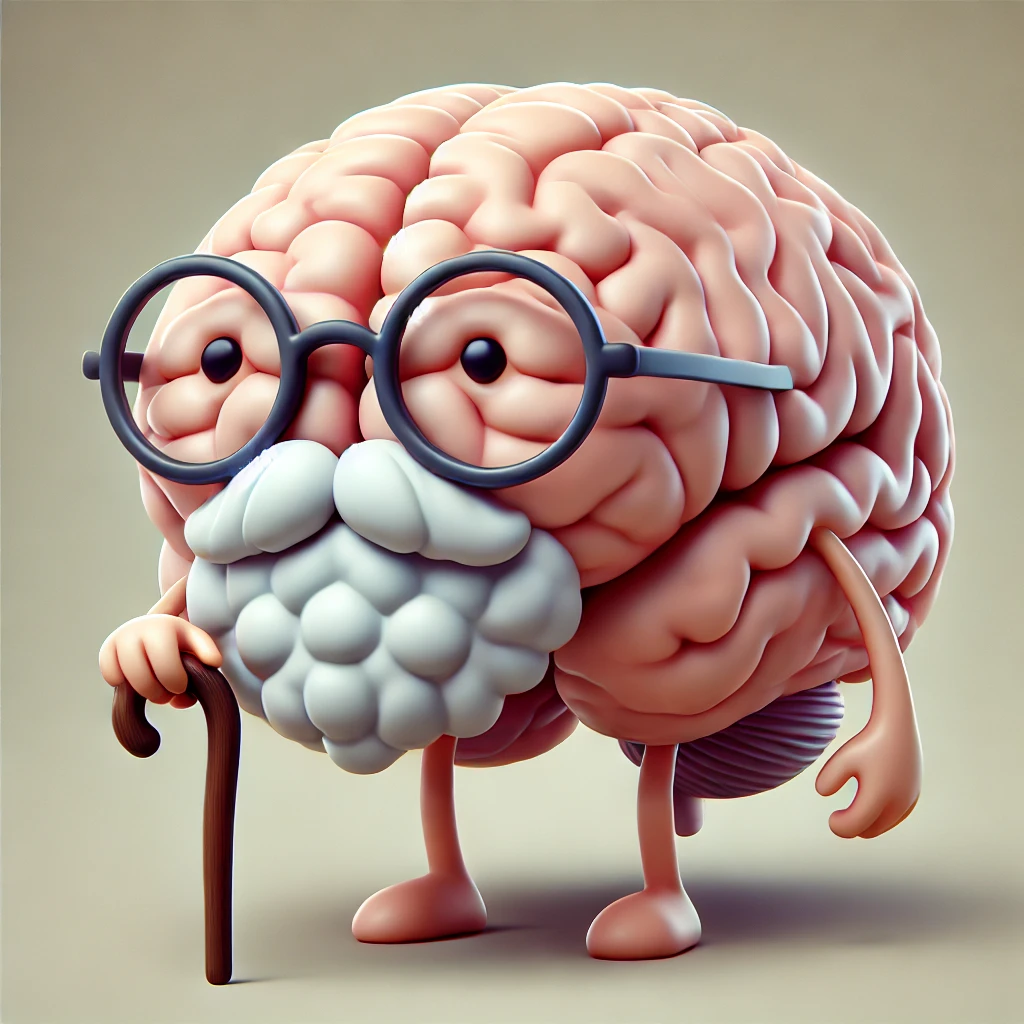
\includegraphics[width=4cm]{data/brainage.png}
            };
        }
        \visible<2>{
            \node[anchor=east] at (5.1, -0.43) {
                \usebox{\brainage}
            };
        }
        \visible<3>{
            \node[anchor=east] at (5.1, -0.43) {
                \usebox{\brainagepredictions}
            };
        }
        \visible<4>{
            \node[] at (0, 0) {
                \hspace{-2.7cm}
                \brainagedataset
            };
        }
        \visible<5>{
            \node[] at (0, 0) {
                \cnnbox{0}
            };
        }
        \visible<6>{
            \node[] at (0, 0) {
                \brainageresults
            };
        }
    \end{tikzpicture}
\end{frame}